\section{Resultados}
\label{sec:resultados}

\subsection{Resultado principal: o gradiente escolaridade--exposição}

As estimativas baseline (Tabela~\ref{tab:gradiente}, coluna 1) indicam um gradiente educacional positivo e significante no nível do indivíduo, com controles mincerianos (idade, idade ao quadrado, gênero e raça) e erros-padrão agrupados por ocupação (122 grupos). O coeficiente de S1 é $\hat{\beta}_1 = 0{,}23$ (erro-padrão 0{,}03; $p < 0{,}001$; $R^2 = 0{,}246$; $N = 227.629$): cada ano adicional de escolaridade associa-se a 0{,}23 ponto a mais de exposição à IA. A magnitude é economicamente relevante: a diferença entre a conclusão do ensino fundamental (8 anos) e do ensino superior (16 anos) implica um acréscimo de cerca de 1{,}84 ponto no escore de exposição tecnológica.

\begin{table}[htbp]
\centering
\caption{Gradiente escolaridade--exposição no nível individual. Variável dependente: exposição à IA da ocupação (0--10). Erros-padrão agrupados por ocupação entre parênteses. Controles mincerianos completos (idade, idade$^2$, gênero e raça) incluídos em todas as colunas. * 10\%, ** 5\%, *** 1\%.}
\label{tab:gradiente}
\begin{tabular}{lcc}
\toprule
 & (1) & (2) \\
 & Baseline (S1) & Rendimento (S2) \\
\midrule
% AUTO-GERADO por scripts/R/04_tables.R — nao editar a mao
Anos de estudo & 0,2288*** & 0,2097*** \\
 & (0,0278) & (0,0260) \\[4pt]
Rendimento habitual (R\$ mil) & -- & 0,0427*** \\
 &  & (0,0100) \\[4pt]
Mulher & 0,051 & 0,113 \\
 & (0,310) & (0,300) \\[4pt]
Idade & -0,0399* & -0,0473** \\
 & (0,0235) & (0,0234) \\[4pt]
$\text{Idade}^2 / 1000$ & 0,4900** & 0,5425** \\[4pt]
 & (0,2257) & (0,2245) \\[4pt]
\midrule
Controles de cor/ra\c{c}a & Sim & Sim \\
Observa\c{c}\~oes & 227.629 & 227.629 \\
$R^2$ & 0,246 & 0,259 \\
Clusters (ocupa\c{c}\~ao) & 122 & 122
 \\
\bottomrule
\end{tabular}
\end{table}

A coluna (2) inclui o rendimento habitual do trabalhador: o coeficiente de escolaridade permanece estável em 0{,}21 (erro-padrão 0{,}03), enquanto o rendimento exibe coeficiente de 0{,}043 por R\$ 1.000 ($p < 0{,}001$). O gradiente educacional não se dissolve com o controle salarial, sugerindo que a escolaridade captura a alocação a conteúdos intrínsecos de tarefas cognitivas, consistente com a Proposição~\ref{prop:gradiente}. O cálculo formal dos limites de \citet{oster2019unobservable} sob $R_{\max} = 1{,}3 R^2$ revela um parâmetro de estabilidade $\delta = 1{,}64 > 1$ ($\beta^*(\delta=1) = 0{,}082$), confirmando que a seleção em não observáveis precisaria ser 64\% superior a toda a seleção em covariáveis mincerianas observáveis para anular o gradiente positivo.\footnote{Conforme preconizado por \citet{oster2019unobservable}, o teto $R_{\max} = 1{,}3 \tilde{R}^2$ constitui o benchmark empírico padrão para dados de pesquisas domiciliares, dado que o limite teórico $R_{\max} = 1{,}0$ ignora o componente idiossincrático e erros de mensuração inerentes aos microdados transversais.} A Figura~\ref{fig:gradiente} ilustra o gradiente na forma de dispersão ponderada.

\begin{figure}[htbp]
\centering

\includegraphics[width=0.85\textwidth]{figures/fig1_gradiente}
\caption{Gradiente escolaridade--exposição. Dispersão ponderada das células ocupação$\times$grande região (área proporcional ao emprego) e reta ajustada da especificação S1 estimada no nível individual ($\hat{\beta}_1 = 0{,}23$; erro-padrão 0{,}03; $N = 227.629$; quadro: intervalo de confiança de 95\% com erros-padrão agrupados por ocupação).}
\label{fig:gradiente}
\end{figure}

\subsection{Exposição e informalidade: mediação e composição educacional}

Em consonância com a Proposição~\ref{prop:formalidade} e o Corolário~\ref{cor:mediacao} (Tabela~\ref{tab:s3}), na especificação incondicional da coluna (1), cada ponto de exposição à IA associa-se a $-6{,}23$ pontos percentuais de probabilidade de informalidade (erro-padrão 0{,}99; $p < 0{,}001$). Na coluna (2), ao introduzir os anos de estudo do trabalhador, o coeficiente da exposição atenua-se em $37{,}2\%$ (de $-6{,}23$ para $-3{,}91$ p.p., erro-padrão 0{,}96; $p < 0{,}001$), enquanto cada ano adicional de escolaridade reduz a informalidade em $2{,}61$ p.p. ($p < 0{,}001$).

\begin{table}[htbp]
\centering
\caption{Informalidade, exposição à IA e escolaridade. Variável dependente: probabilidade de informalidade (p.p.). Estimativas por WLS com pesos amostrais da PNAD Contínua. Erros-padrão agrupados por ocupação entre parênteses. Controles mincerianos incluídos em ambas as colunas. * 10\%, ** 5\%, *** 1\%.}
\label{tab:s3}
\begin{tabular}{lcc}
\toprule
 & (1) & (2) \\
 & Incondicional (S3a) & Condicional (S3) \\
\midrule
% AUTO-GERADO por scripts/R/04_tables.R — nao editar a mao
Exposi\c{c}\~ao \`a IA ($\theta_j$) & -6,228*** & -3,907*** \\
 & (0,987) & (0,957) \\[4pt]
Anos de estudo & -- & -2,609*** \\
 &  & (0,270) \\[4pt]
Mulher & 1,579 & 3,878 \\
 & (3,003) & (2,780) \\[4pt]
Idade & -2,363*** & -2,025*** \\
 & (0,219) & (0,215) \\[4pt]
\midrule
Controles Mincerianos & Sim & Sim \\
Observa\c{c}\~oes & 227.629 & 227.629 \\
$R^2$ & 0,080 & 0,108 \\
Clusters (ocupa\c{c}\~ao) & 122 & 122
 \\
\bottomrule
\end{tabular}
\end{table}

Essa atenuação é consistente com o fato de que a relação bruta observada entre exposição e formalidade é substancialmente mediada pela composição de capital humano: postos de trabalho altamente expostos concentram-se no setor formal em grande parte porque empregam indivíduos com elevada escolaridade, cujas tarefas cognitivas complementam a tecnologia. Ao mesmo tempo, o fato de $\hat{\delta}_1$ reter $62{,}8\%$ de sua magnitude inicial de forma estatisticamente significante corrobora a previsão de mediação parcial do Corolário~\ref{cor:mediacao}: para além do atributo educacional do trabalhador, a exposição captura o canal ocupacional direto, decorrente de requisitos organizacionais, escala e capital complementar próprios de firmas formais.\footnote{Em termos de forma funcional, a estimação de um modelo logístico ponderado (\emph{WLS logit}) gera efeitos marginais médios (AME) estritamente equivalentes em sinal e atenuação percentual ao modelo de probabilidade linear, garantindo que o resultado não decorre de restrições de suporte no espaço de probabilidades.} A Figura~\ref{fig:mediacao} resume o contraste em dois painéis: associação bruta (Painel A, S3a) e parcial (Painel B, S3, condicionada à escolaridade e aos controles mincerianos).

\begin{figure}[htbp]
\centering
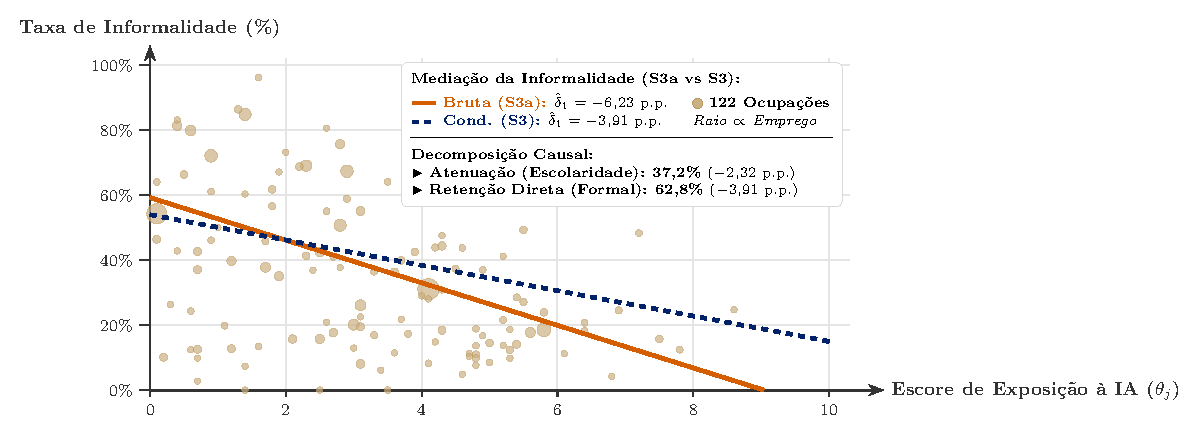
\includegraphics[width=0.85\textwidth]{figures/fig2_mediacao}
\caption{Mediação pela escolaridade da associação exposição--informalidade. Painel A: relação bruta (S3a, $\hat{\delta}_1 = -6{,}23$ p.p.; erro-padrão 0{,}99). Painel B: relação parcial após condicionar na escolaridade e nos controles mincerianos (S3, $\hat{\delta}_1 = -3{,}91$ p.p.; erro-padrão 0{,}96). A atenuação de $37{,}2\%$ do coeficiente é consistente com a mediação parcial do Corolário~\ref{cor:mediacao}.}
\label{fig:mediacao}
\end{figure}

\subsection{Heterogeneidade regional nas 27 Unidades da Federação}

A interação entre escolaridade individual e formalidade média da UF confirma a heterogeneidade espacial prevista pela teoria (Tabela~\ref{tab:s4}): o termo de interação é positivo e expressivo ($\hat{\beta}_2 = 0{,}28$; erro-padrão 0{,}06; $p < 0{,}001$), acompanhado de um efeito principal da formalidade regional de $\hat{\beta}_3 = -3{,}10$ (erro-padrão 0{,}77; $p < 0{,}001$).

\begin{table}[htbp]
\centering
\caption{Gradiente escolaridade--exposição por profundidade formal da UF (27 UFs). Variável dependente: exposição à IA (0--10). Estimativas por WLS com pesos amostrais. Formalidade da UF calculada via \emph{leave-one-out}; erros-padrão agrupados por ocupação. Controles mincerianos incluídos. * 10\%, ** 5\%, *** 1\%.}
\label{tab:s4}
\begin{tabular}{lc}
\toprule
 & (1) \\
 & Interação Regional (S4) \\
\midrule
% AUTO-GERADO por scripts/R/04_tables.R — nao editar a mao
Anos de estudo ($e_i$) & 0,0681** \\
 & (0,0326) \\[4pt]
Escolaridade $\times$ Formalidade Regional & 0,2786*** \\
 & (0,0649) \\[4pt]
Taxa de Formalidade Regional (LOO) & -3,104*** \\
 & (0,767) \\[4pt]
\midrule
Limiar cr\'itico de polariza\c{c}\~ao ($e^*$) & 11,14 anos \\
Controles Mincerianos & Sim \\
Observa\c{c}\~oes & 227.629 \\
$R^2$ & 0,250 \\
Clusters (ocupa\c{c}\~ao) & 122
 \\
\bottomrule
\end{tabular}
\end{table}

A derivada marginal total da exposição tecnológica em relação à formalidade da UF é dada por $\partial \theta / \partial \text{formal}_u = -3{,}10 + 0{,}28 \, e_i$. Esse resultado aponta para uma dinâmica de polarização ocupacional no espaço geográfico: para trabalhadores com baixa escolaridade ($e_i < 11$ anos), maior maturidade formal regional associa-se a menor exposição média (ex.: $-0{,}86$ ponto para o ensino fundamental de 8 anos), refletindo a substituição de rotinas de suporte informal por processos estruturados; em contrapartida, para trabalhadores altamente qualificados ($e_i = 16$ anos), o efeito é fortemente positivo ($+1{,}38$ ponto).\footnote{A inferência de S4 é igualmente robusta à clusterização bidirecional (\emph{two-way clustering} por ocupação e UF), que produz erros-padrão indistinguíveis da clusterização ocupacional baseline.} Assim, mercados regionais com maior densidade formal ampliam a distância de exposição entre o topo e a base educacional. Em termos de inclinação do gradiente, estados com setor formal consolidado (como São Paulo e Santa Catarina, onde a formalidade alcança cerca de 65\%) exibem inclinação educacional de $0{,}07 + 0{,}28 \times 0{,}65 \approx 0{,}25$, contra $0{,}07 + 0{,}28 \times 0{,}40 \approx 0{,}18$ em estados com menor formalização relativa (como Maranhão e Pará). A Figura~\ref{fig:regional} ilustra o gradiente por grande região.

\begin{figure}[htbp]
\centering

\includegraphics[width=0.85\textwidth]{figures/fig3_regional_slopes}
\caption{Gradiente escolaridade--exposição por grande região. Cada reta ajusta as células ocupação$\times$UF dentro da região (ponderadas pelo emprego); a legenda reporta a taxa de formalidade regional e a inclinação estimada. O gradiente é mais íngreme nas regiões de setor formal mais profundo, em consonância com a Proposição~\ref{prop:regiao}.}
\label{fig:regional}
\end{figure}

\subsection{Robustez econométrica}
\label{subsec:robustez}

O gradiente estimado permanece inalterado sob uma bateria abrangente de sensibilidade que avalia potenciais ameaças de estratificação amostral, não-linearidade e influência de ocupações de cauda (Tabela~\ref{tab:robustez}). Sem ponderação amostral (OLS simples), o coeficiente é 0{,}21 (erro-padrão 0{,}03), atestando que a estratificação amostral não gera artificialmente o gradiente. O tratamento de valores extremos --- winsorização a 1\%/99\% ou exclusão de observações com exposição no percentil superior ($N = 225.478$) --- preserva estimativas virtualmente inalteradas de 0{,}23 e 0{,}22, respectivamente, descartando que o efeito seja puxado por elites tecnológicas concentradas. Com a transformação não linear $\log(1+\theta)$, o coeficiente é 0{,}07 (erro-padrão 0{,}01; $p < 0{,}001$), cujo efeito marginal avaliado na média amostral ($\approx 0{,}27$) corrobora a especificação linear.

\begin{table}[htbp]
\centering
\caption{Robustez do gradiente escolaridade--exposição no nível individual. Variável dependente: exposição à IA (0--10); na coluna (5), $\log(1+\theta)$. Coluna (1): baseline WLS. Coluna (2): OLS não ponderado. Coluna (3): exposição winsorizada a 1\%/99\%. Coluna (4): exclusão de observações com exposição acima do percentil 99. Erros-padrão agrupados por ocupação entre parênteses. Controles mincerianos incluídos. * 10\%, ** 5\%, *** 1\%.}
\label{tab:robustez}
\begin{tabular}{lccccc}
\toprule
 & (1) & (2) & (3) & (4) & (5) \\
 & WLS Baseline & OLS Simples & Winsor. 1\% & Excl. p99 & $\log(1+\theta)$ \\
\midrule
% AUTO-GERADO por scripts/R/04_tables.R — nao editar a mao
Anos de escolaridade & 0,23*** & 0,21*** & 0,23*** & 0,23*** & 0,07*** \\
 & (0,03) & (0,03) & (0,03) & (0,03) & (0,01) \\[4pt]
Constante & 1,10* & 1,11* & 1,10* & 1,14* & 0,70*** \\
 & (0,60) & (0,59) & (0,60) & (0,60) & (0,18) \\
\midrule
$R^2$ & 0,25 & 0,24 & 0,25 & 0,24 & 0,24 \\
$N$ (indiv\'iduos) & 227.629 & 227.629 & 227.629 & 225.390 & 227.629
 \\
\bottomrule
\end{tabular}
\end{table}

A exclusão sequencial de cada um dos 9 grandes grupos ocupacionais da COD (Tabela~\ref{tab:robustezgrupos} no Apêndice) mostra que o gradiente se mantém entre 0{,}19 e 0{,}26 em todas as subamostras. Para a dimensão regional (S4), a inferência estatística sob a estrutura das 27 UFs é corroborada pelo teste de \emph{wild cluster bootstrap} \citep{cameron2008bootstrap} com 1.000 replicações ($p < 0{,}001$), confirmando que a significância do termo de interação regional é imune a dependências espaciais em múltiplos níveis. A Figura~\ref{fig:robustez} resume os coeficientes e intervalos de confiança em gráfico de floresta.

\begin{figure}[htbp]
\centering

\includegraphics[width=0.85\textwidth]{figures/fig5_robustez_forest}
\caption{Robustez do gradiente escolaridade--exposição. Coeficiente $\hat{\beta}_1$ e intervalos de confiança de 95\% (erros-padrão agrupados por ocupação) na especificação baseline (S1), nas exclusões sequenciais de cada grande grupo ocupacional e nas variantes de amostra e ponderação: \emph{OLS} não ponderado, winsorização a 1\%/99\% e exclusão do percentil superior ($N = 225.478$).}
\label{fig:robustez}
\end{figure}
